\documentclass[conference]{IEEEtran}
\usepackage{cite}
\usepackage{amsmath,amssymb,amsfonts}
\usepackage{algorithmic}
\usepackage{graphicx}
\usepackage{textcomp}
\usepackage{xcolor}
\usepackage{booktabs}
\usepackage{multirow}
\usepackage{url}
\usepackage{hyperref}
% \usepackage{svg} % Requires Inkscape - using placeholders for SVG figures
\graphicspath{{figures/}{paper_charts/}}

\def\BibTeX{{\rm B\kern-.05em{\sc i\kern-.025em b}\kern-.08em
    T\kern-.1667em\lower.7ex\hbox{E}\kern-.125emX}}

\begin{document}

\title{An AI-Powered IELTS Preparation Platform with Event-Driven Architecture and Local Speech Processing}

\author{
\IEEEauthorblockN{[Your Full Name]}
\IEEEauthorblockA{Faculty of Information Technology\\
Industrial University of Ho Chi Minh City\\
Email: [your-email]@iuh.edu.vn}
}

\maketitle

\begin{abstract}
The International English Language Testing System (IELTS) remains the most widely accepted English proficiency examination globally, yet most existing preparation platforms fail to provide automated feedback for subjective skills such as Writing and Speaking, rely heavily on expensive cloud-based APIs for speech processing, and lack personalized learning pathways. This paper presents IELTS Master English AI, a comprehensive IELTS preparation platform built on an Event-Driven Hybrid Architecture that separates computationally intensive AI inference from core business logic. The system employs a NestJS modular monolith as the core backend, a dedicated Python FastAPI microservice for AI processing, and RabbitMQ as the asynchronous message broker connecting them. Key technical contributions include: (1) local speech-to-text processing using Faster-Whisper, eliminating per-request cloud API costs; (2) LLM-based automated Writing and Speaking grading with structured rubric output following official IELTS band descriptors; (3) an SM-2 spaced repetition vocabulary system with custom card types; and (4) a personalized learning roadmap driven by onboarding diagnostics. Experimental evaluation demonstrates that the SM-2 algorithm effectively differentiates user proficiency through adaptive interval scheduling, and the Levenshtein-based pronunciation scoring provides discriminative capability across difficulty levels.
\end{abstract}

\begin{IEEEkeywords}
IELTS preparation, Event-driven architecture, Speech-to-text, Automated essay scoring, Spaced repetition, NestJS, FastAPI
\end{IEEEkeywords}

% ============================================================
\section{Introduction}
% ============================================================

The International English Language Testing System (IELTS) is recognized by over 11,000 organizations across 140 countries, making it the world's most popular English proficiency test for higher education and migration purposes \cite{ielts_stats}. With the global surge in online learning, the demand for accessible, AI-driven IELTS preparation tools has increased dramatically. However, a critical analysis of existing platforms reveals several persistent limitations.

First, most commercial applications such as Duolingo and ELSA Speak focus on general English proficiency rather than IELTS-specific exam preparation. They lack structured mock examinations covering all four IELTS skills --- Listening, Reading, Writing, and Speaking --- in a single integrated environment. Second, automated grading for subjective skills remains a significant technical challenge. While Reading and Listening can be graded deterministically against answer keys, Writing and Speaking require nuanced evaluation of grammar, vocabulary, coherence, and pronunciation --- traditionally requiring human examiners. Third, platforms that do incorporate speech analysis typically rely on cloud-based Speech-to-Text APIs (e.g., Google Cloud Speech, Amazon Transcribe), introducing per-request costs, latency variability, and external dependency. Fourth, existing solutions rarely offer personalized learning pathways that adapt to individual learner goals, daily time commitments, and current proficiency levels.

To address these challenges, this paper introduces IELTS Master English AI, a full-stack educational platform engineered specifically for comprehensive IELTS preparation. The system is built upon the following key contributions:

\begin{itemize}
    \item An \textbf{Event-Driven Hybrid Architecture} that decouples AI inference workloads from core business logic using RabbitMQ as the message broker, ensuring the web interface never blocks during computationally intensive operations.
    \item \textbf{Local speech-to-text processing} using Faster-Whisper \cite{faster_whisper}, a CTranslate2-optimized implementation of OpenAI's Whisper model, eliminating per-request cloud API costs while maintaining competitive accuracy.
    \item \textbf{LLM-based automated IELTS Writing and Speaking grading} using Llama 3.3 70B, with strictly enforced JSON output schemas following official IELTS band descriptors across four criteria per skill.
    \item An \textbf{SM-2 spaced repetition vocabulary system} (Vocab Lab) with customizable card types, field definitions, and templates.
    \item A \textbf{personalized learning roadmap} generated from onboarding diagnostics, with sequential step-level locking to enforce structured progression.
\end{itemize}

The remainder of this paper is organized as follows. Section~II presents the theoretical background and key algorithms. Section~III provides a comparative analysis with existing platforms. Section~IV details the system architecture and design. Section~V describes the implementation and experimental evaluation. Section~VI concludes with a summary and future work directions.

% ============================================================
\section{Theoretical Background}
% ============================================================

\subsection{Event-Driven Architecture}
An event-driven architecture (EDA) is a software design pattern in which the flow of the program is determined by events --- messages published to and consumed from a message broker. In educational platforms that integrate AI/ML inference, EDA is particularly valuable because operations such as speech transcription (2--10 seconds) and LLM-based essay evaluation (5--30 seconds) would otherwise block the main API thread, degrading user experience \cite{richards_arch}.

\subsection{NestJS Framework}
NestJS is a progressive Node.js framework built with TypeScript that employs a modular architecture inspired by Angular. It provides dependency injection, decorators, guards, and interceptors, enabling the construction of scalable server-side applications \cite{nestjs_docs}. The framework naturally supports the Modular Monolith pattern.

\subsection{FastAPI Framework}
FastAPI is a modern, high-performance Python web framework designed for building APIs. Its native async/await support makes it well-suited for I/O-bound AI inference tasks \cite{fastapi_docs}.

\subsection{Faster-Whisper for Speech-to-Text}
Faster-Whisper \cite{faster_whisper} is a reimplementation of OpenAI's Whisper model \cite{whisper_paper} using CTranslate2. It provides up to 4$\times$ faster inference with comparable accuracy. The system uses beam search ($\text{beam\_size}=5$) and Voice Activity Detection (VAD) filtering.

\subsection{LLM-Based Automated Grading}
Large Language Models can be instructed to evaluate text against structured rubrics \cite{gpt3}. This system uses Llama 3.3 70B with system prompts enforcing band score assignment, structured JSON output, and specific mistake identification. The overall Writing band is calculated as:
\begin{equation}
    \text{Overall} = \frac{\text{Task1\_Band} + \text{Task2\_Band} \times 2}{3}
\end{equation}

\subsection{SM-2 Spaced Repetition Algorithm}
The SM-2 algorithm, developed by Wozniak \cite{sm2}, optimizes long-term memory retention. Given a quality rating $q \in \{0, 1, 2, 3, 4, 5\}$, the ease factor is updated:
\begin{equation}
    EF' = EF + (0.1 - (5-q) \times (0.08 + (5-q) \times 0.02))
\end{equation}
where $EF \geq 1.3$. The review interval follows:
\begin{equation}
    I(n) = \begin{cases} 1 & \text{if } n = 1 \\ 6 & \text{if } n = 2 \\ I(n-1) \times EF & \text{if } n > 2 \end{cases}
\end{equation}
If $q < 3$, the repetition counter resets to 0.

\subsection{Levenshtein Distance for Pronunciation Scoring}
Pronunciation accuracy is measured using a Levenshtein distance variant \cite{levenshtein}:
\begin{equation}
    \text{Score} = \left(1 - \frac{d(T, W)}{\max(|T|, |W|)}\right) \times 100
\end{equation}
where $d(T, W)$ is the minimum edit distance between transcription $T$ and target word $W$.

\subsection{IELTS Answer Matching}
For Reading and Listening, the system implements flexible matching handling alternative answers (``/''), optional words (parentheses), and case-insensitive comparison.

% ============================================================
\section{Related Work and System Comparison}
% ============================================================

Table~\ref{tab:comparison} compares IELTS Master AI with four representative platforms.

\begin{table*}[htbp]
\caption{Feature Comparison of Language Learning Platforms}
\label{tab:comparison}
\centering
\begin{tabular}{lccccc}
\toprule
\textbf{Feature} & \textbf{IELTS Master AI} & \textbf{Duolingo} & \textbf{ELSA Speak} & \textbf{Cambridge} & \textbf{SLP \cite{reference_paper}} \\
\midrule
IELTS Mock Exams (4-skill) & \checkmark & -- & -- & Limited & -- \\
AI Writing Grading & LLM rubric & -- & -- & -- & Gemini basic \\
AI Speaking Grading & Whisper + LLM & -- & Phoneme & -- & -- \\
Pronunciation Checker & Local Whisper & -- & Cloud API & -- & Cloud API \\
SM-2 Spaced Repetition & \checkmark & -- & -- & -- & -- \\
Shadowing/Dictation & YouTube-based & -- & -- & -- & -- \\
Event-Driven AI & RabbitMQ & -- & -- & -- & -- \\
Personalized Roadmap & Onboarding & Placement & -- & -- & AI-generated \\
Real Exam Content & Cambridge 14--20 & -- & -- & \checkmark & -- \\
Cross-Platform & Web + Mobile & Web + Mobile & Mobile & Mobile & Web + Mobile \\
\bottomrule
\end{tabular}
\end{table*}

Key differentiators include: (1) \textbf{Event-Driven AI Processing} ensuring sub-second API responses during heavy inference; (2) \textbf{Local Speech Processing} eliminating cloud API costs; and (3) \textbf{Comprehensive IELTS Coverage} integrating all four skills with authentic Cambridge content.

% ============================================================
\section{System Architecture and Design}
% ============================================================

\subsection{Architecture Overview}
The platform is architected as an Event-Driven Hybrid system with three layers: Client (Next.js 14 + React Native/Expo), Application (NestJS + FastAPI + RabbitMQ on K3s), and Data (PostgreSQL 16 + Redis 7 + MinIO). Fig.~\ref{fig:architecture} illustrates the high-level architecture.

\begin{figure}[htbp]
\centerline{
\includegraphics[width=\columnwidth]{figure_1_system_architecture_overview.png}}
\caption{System architecture overview showing the three-layer Event-Driven Hybrid design.}
\label{fig:architecture}
\end{figure}

\subsection{Database Design}
The data model comprises 35+ Prisma models across domain groupings: Core (User, Exam, ExamSession, Result), IELTS Learning (IeltsSkill, IeltsLesson, exercises), Vocabulary (books, units, words), Vocab Lab (Deck, Flashcard with SM-2 fields, CardType, CardTemplate), Shadowing (ShadowingVideo with timestamps), Grammar, and Pronunciation (PronunciationAttempt with async status tracking). Fig.~\ref{fig:erd} presents the entity-relationship diagram for the key entities.

\begin{figure}[htbp]
\centerline{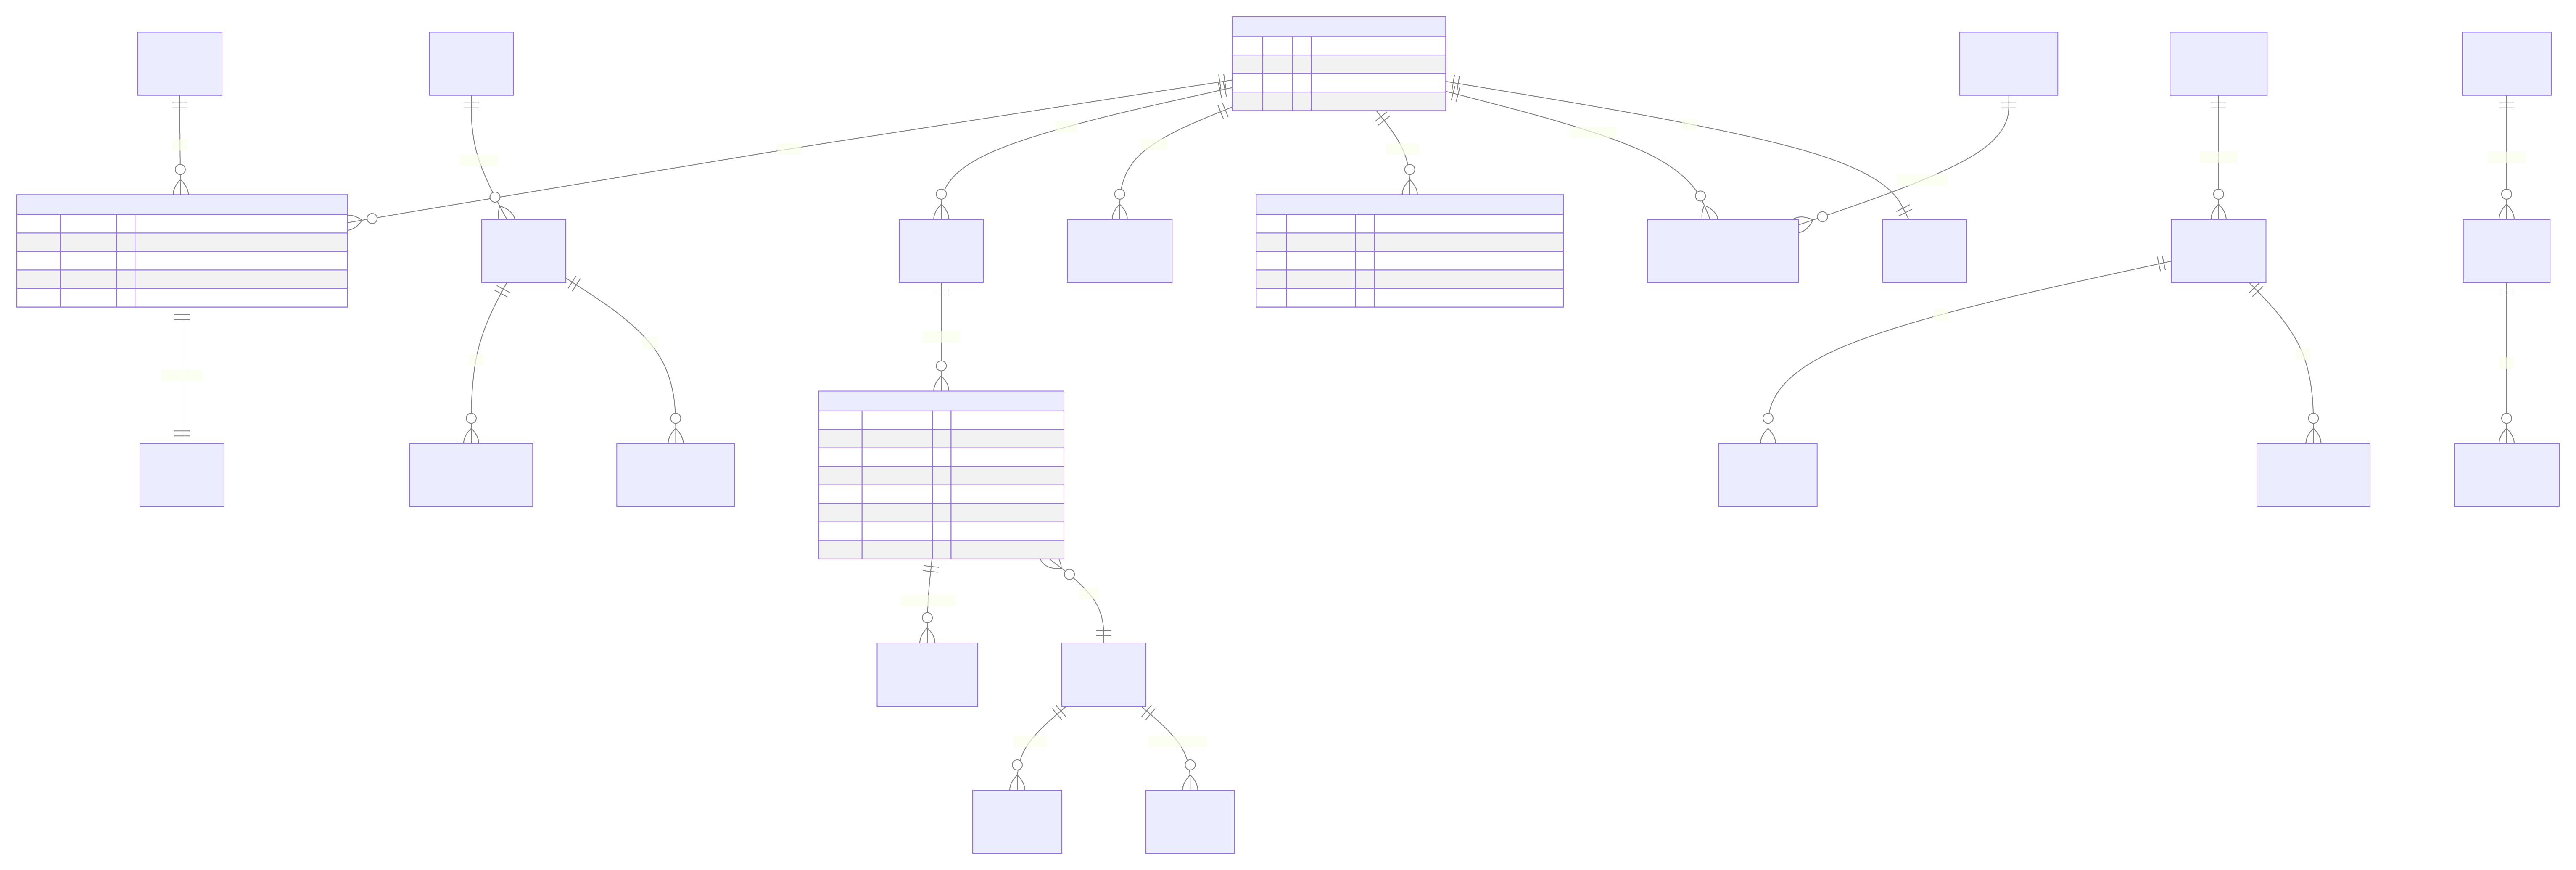
\includegraphics[width=\columnwidth]{figure_2_entity_relationship_diagram_key_entities.png}}
\caption{Entity-relationship diagram showing key domain entities and their associations.}
\label{fig:erd}
\end{figure}

\subsection{Authentication and Authorization}
JWT-based authentication via NestJS Guards with role-based access control (STUDENT, ADMIN, INSTRUCTOR) and Redis session caching.

\subsection{AI-Powered Grading Pipeline}
The AI grading pipeline is the system's most significant technical contribution. Fig.~\ref{fig:grading_pipeline} illustrates the end-to-end AI grading flow.

\begin{figure}[htbp]
\centerline{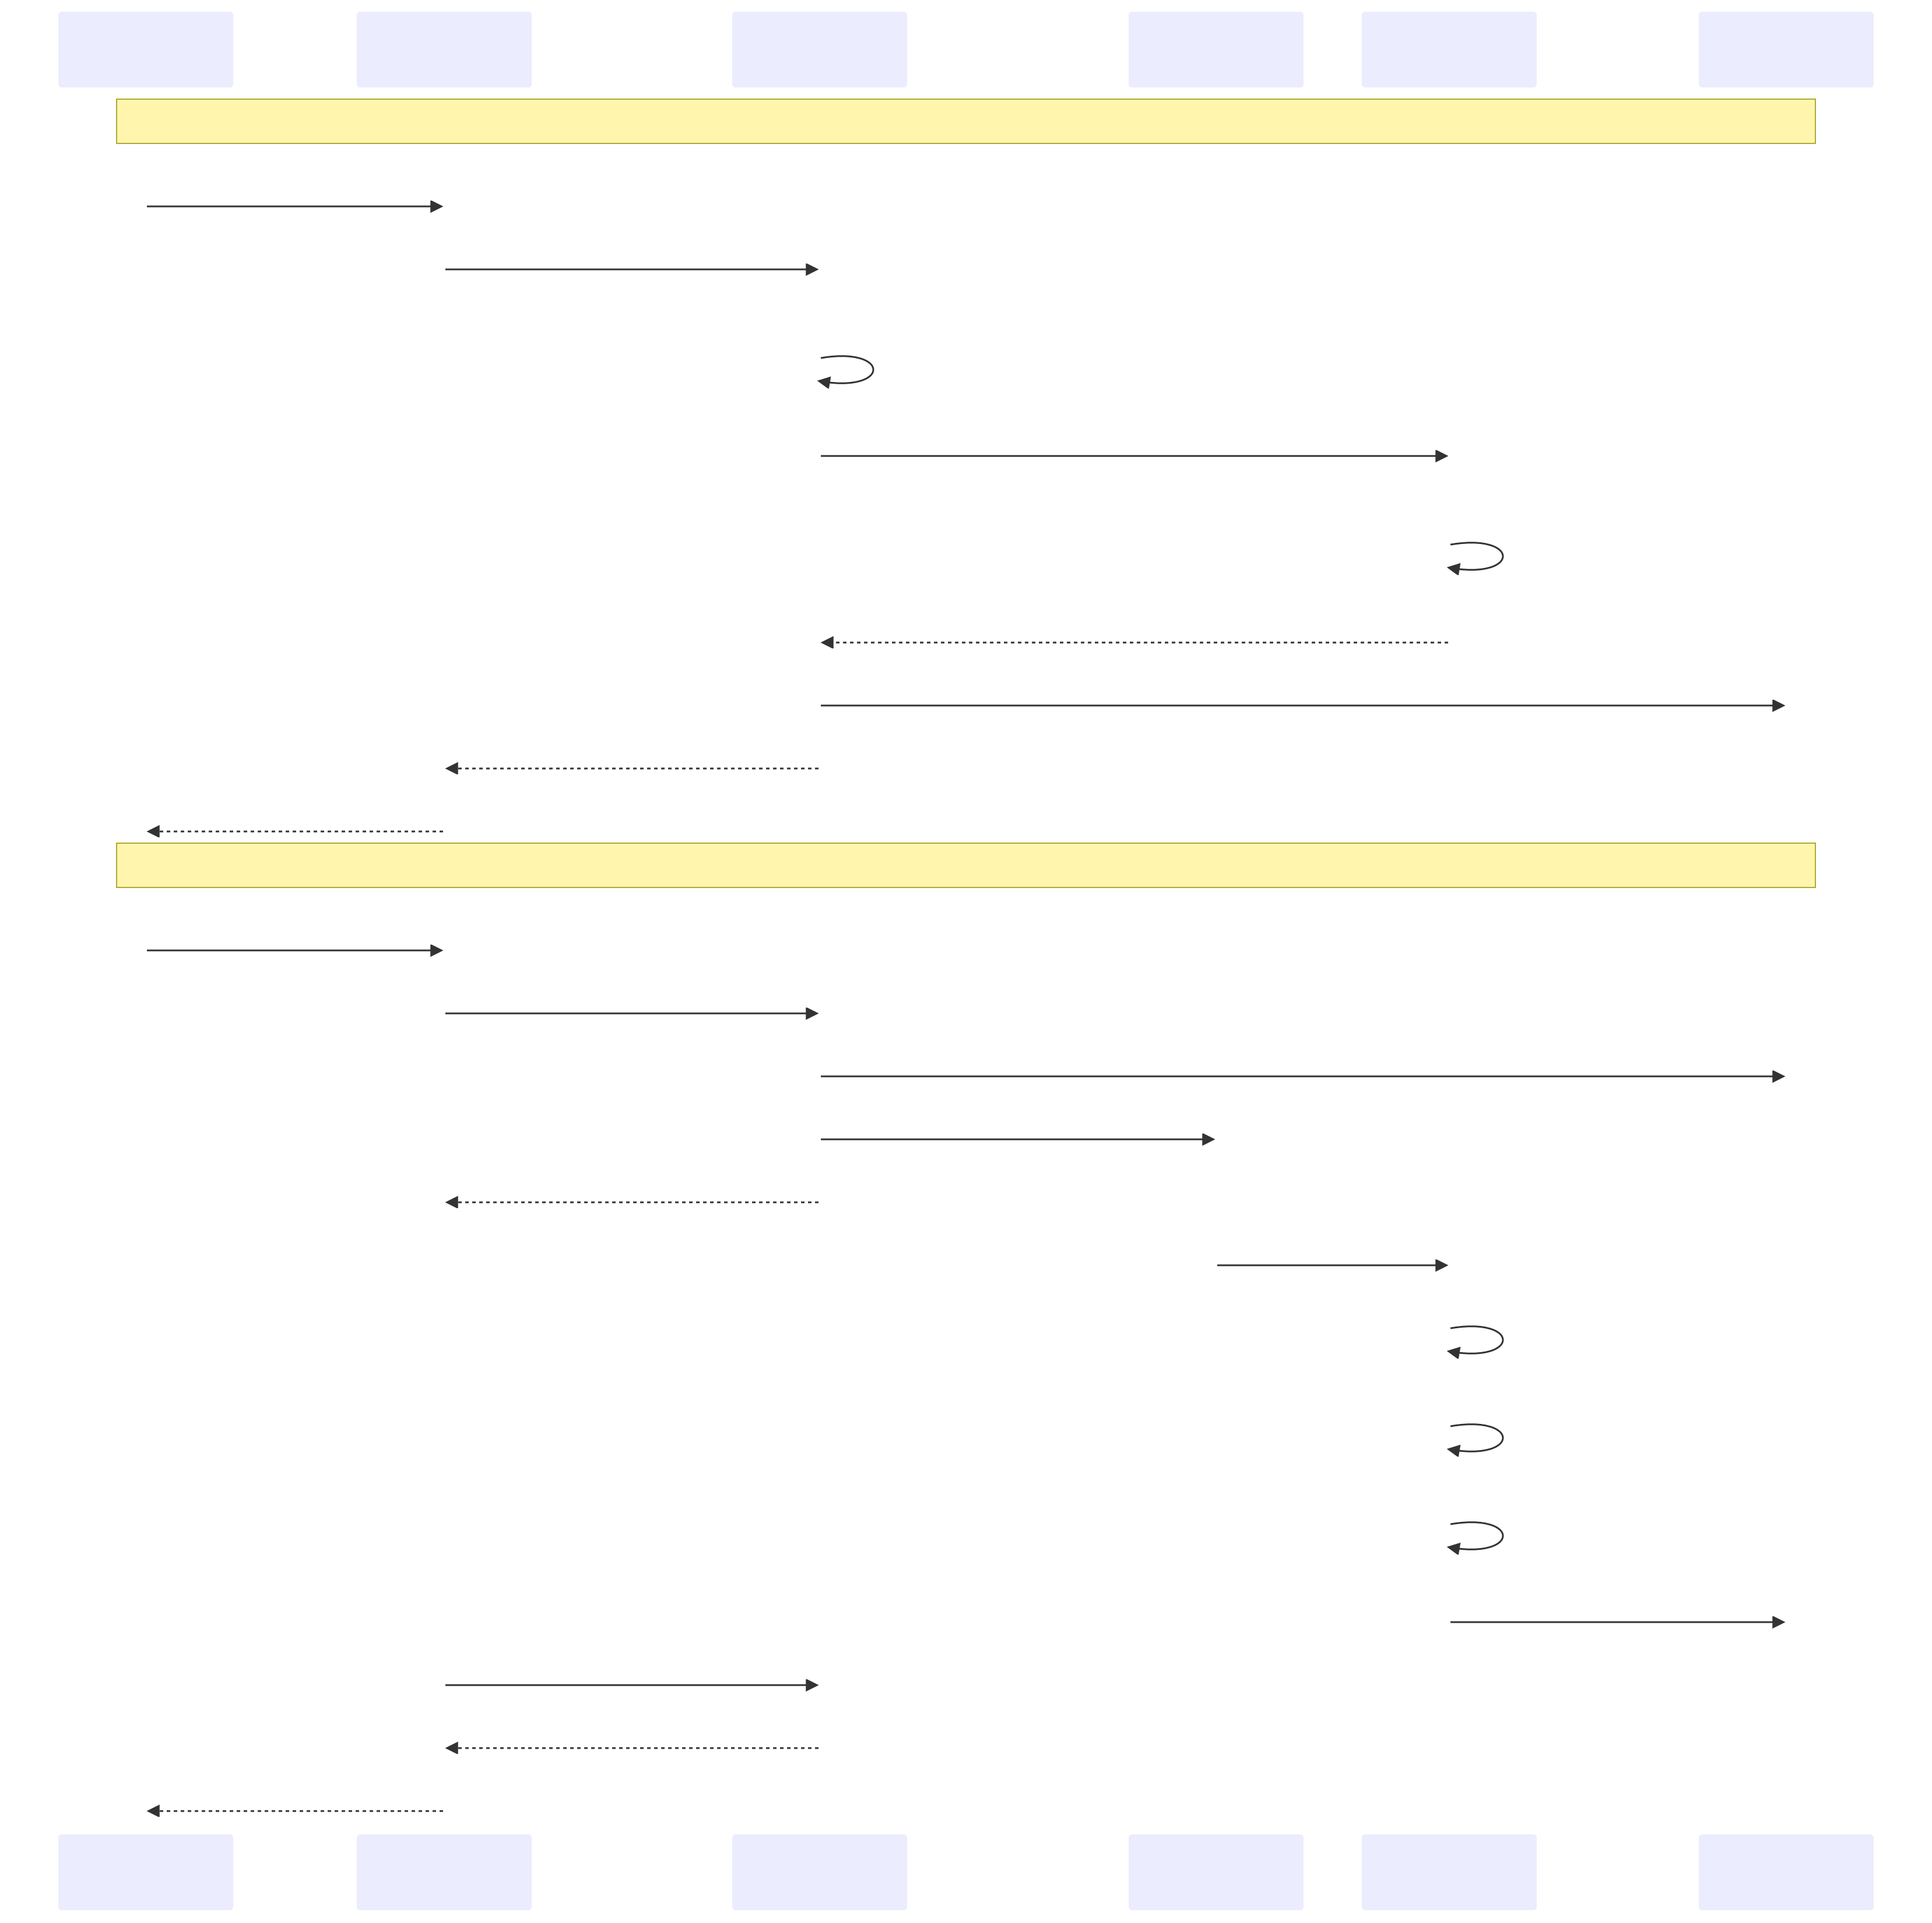
\includegraphics[width=\columnwidth]{figure_3_ai_grading_pipeline.png}}
\caption{AI grading pipeline showing the request flow from client through NestJS, RabbitMQ, and FastAPI for Writing, Speaking, and Pronunciation evaluation.}
\label{fig:grading_pipeline}
\end{figure}

\subsubsection{Writing Grading}
The Core Backend sends a synchronous HTTP request to FastAPI. The AI Service uses Llama 3.3 70B with a system prompt enforcing four IELTS Writing criteria (Task Achievement, Coherence/Cohesion, Lexical Resource, Grammatical Range). The model outputs structured JSON with band scores, strengths, weaknesses, and specific mistakes. Server-side band recalculation ensures consistency via Equation~(1).

\subsubsection{Speaking Grading}
A three-stage pipeline: (1) audio decoding (Base64/URL), (2) Faster-Whisper transcription with VAD, (3) LLM evaluation against four Speaking criteria.

\subsubsection{Pronunciation Checking (Asynchronous)}
Uses the full event-driven pipeline: NestJS publishes to RabbitMQ $\rightarrow$ FastAPI consumer downloads audio from MinIO $\rightarrow$ Whisper transcription $\rightarrow$ Levenshtein scoring (Equation~4) $\rightarrow$ direct PostgreSQL update.

\subsection{IELTS Exam Engine}
Supports deterministic grading for Listening/Reading (flexible answer matching) and AI grading for Writing/Speaking. Session persistence enables Save \& Pause functionality.

\subsection{SM-2 Spaced Repetition Vocab Lab}
Implements the SM-2 algorithm (Equations~2--3) with custom card types, configurable field definitions, front/back templates, and a priority-ordered study queue. Fig.~\ref{fig:sm2_flowchart} shows the SM-2 algorithm decision flowchart.

\begin{figure}[htbp]
\centerline{
\includegraphics[width=\columnwidth]{sm2_algorithm_flowchart.png}}
\caption{SM-2 spaced repetition algorithm flowchart showing the card state transitions and interval calculation logic.}
\label{fig:sm2_flowchart}
\end{figure}

\subsection{Personalized Learning Roadmap}
Generated from onboarding data (target band, daily commitment, placement score). Content is interleaved across skills and chunked into time-budgeted steps with sequential locking.

\subsection{Shadowing and Dictation System}
YouTube video integration with timestamped sentences, per-word IPA phonetics, Vietnamese translations, and four dictation difficulty levels.

% ============================================================
\section{Implementation and Results}
% ============================================================

\subsection{Deployment Architecture}
Local development uses Docker Compose (PostgreSQL 16, Redis 7, RabbitMQ 3, MinIO, PgAdmin). Production deploys on GCP using K3s Kubernetes with Traefik Ingress Controller. Fig.~\ref{fig:deployment} shows the deployment topology.

\begin{figure}[htbp]
\centerline{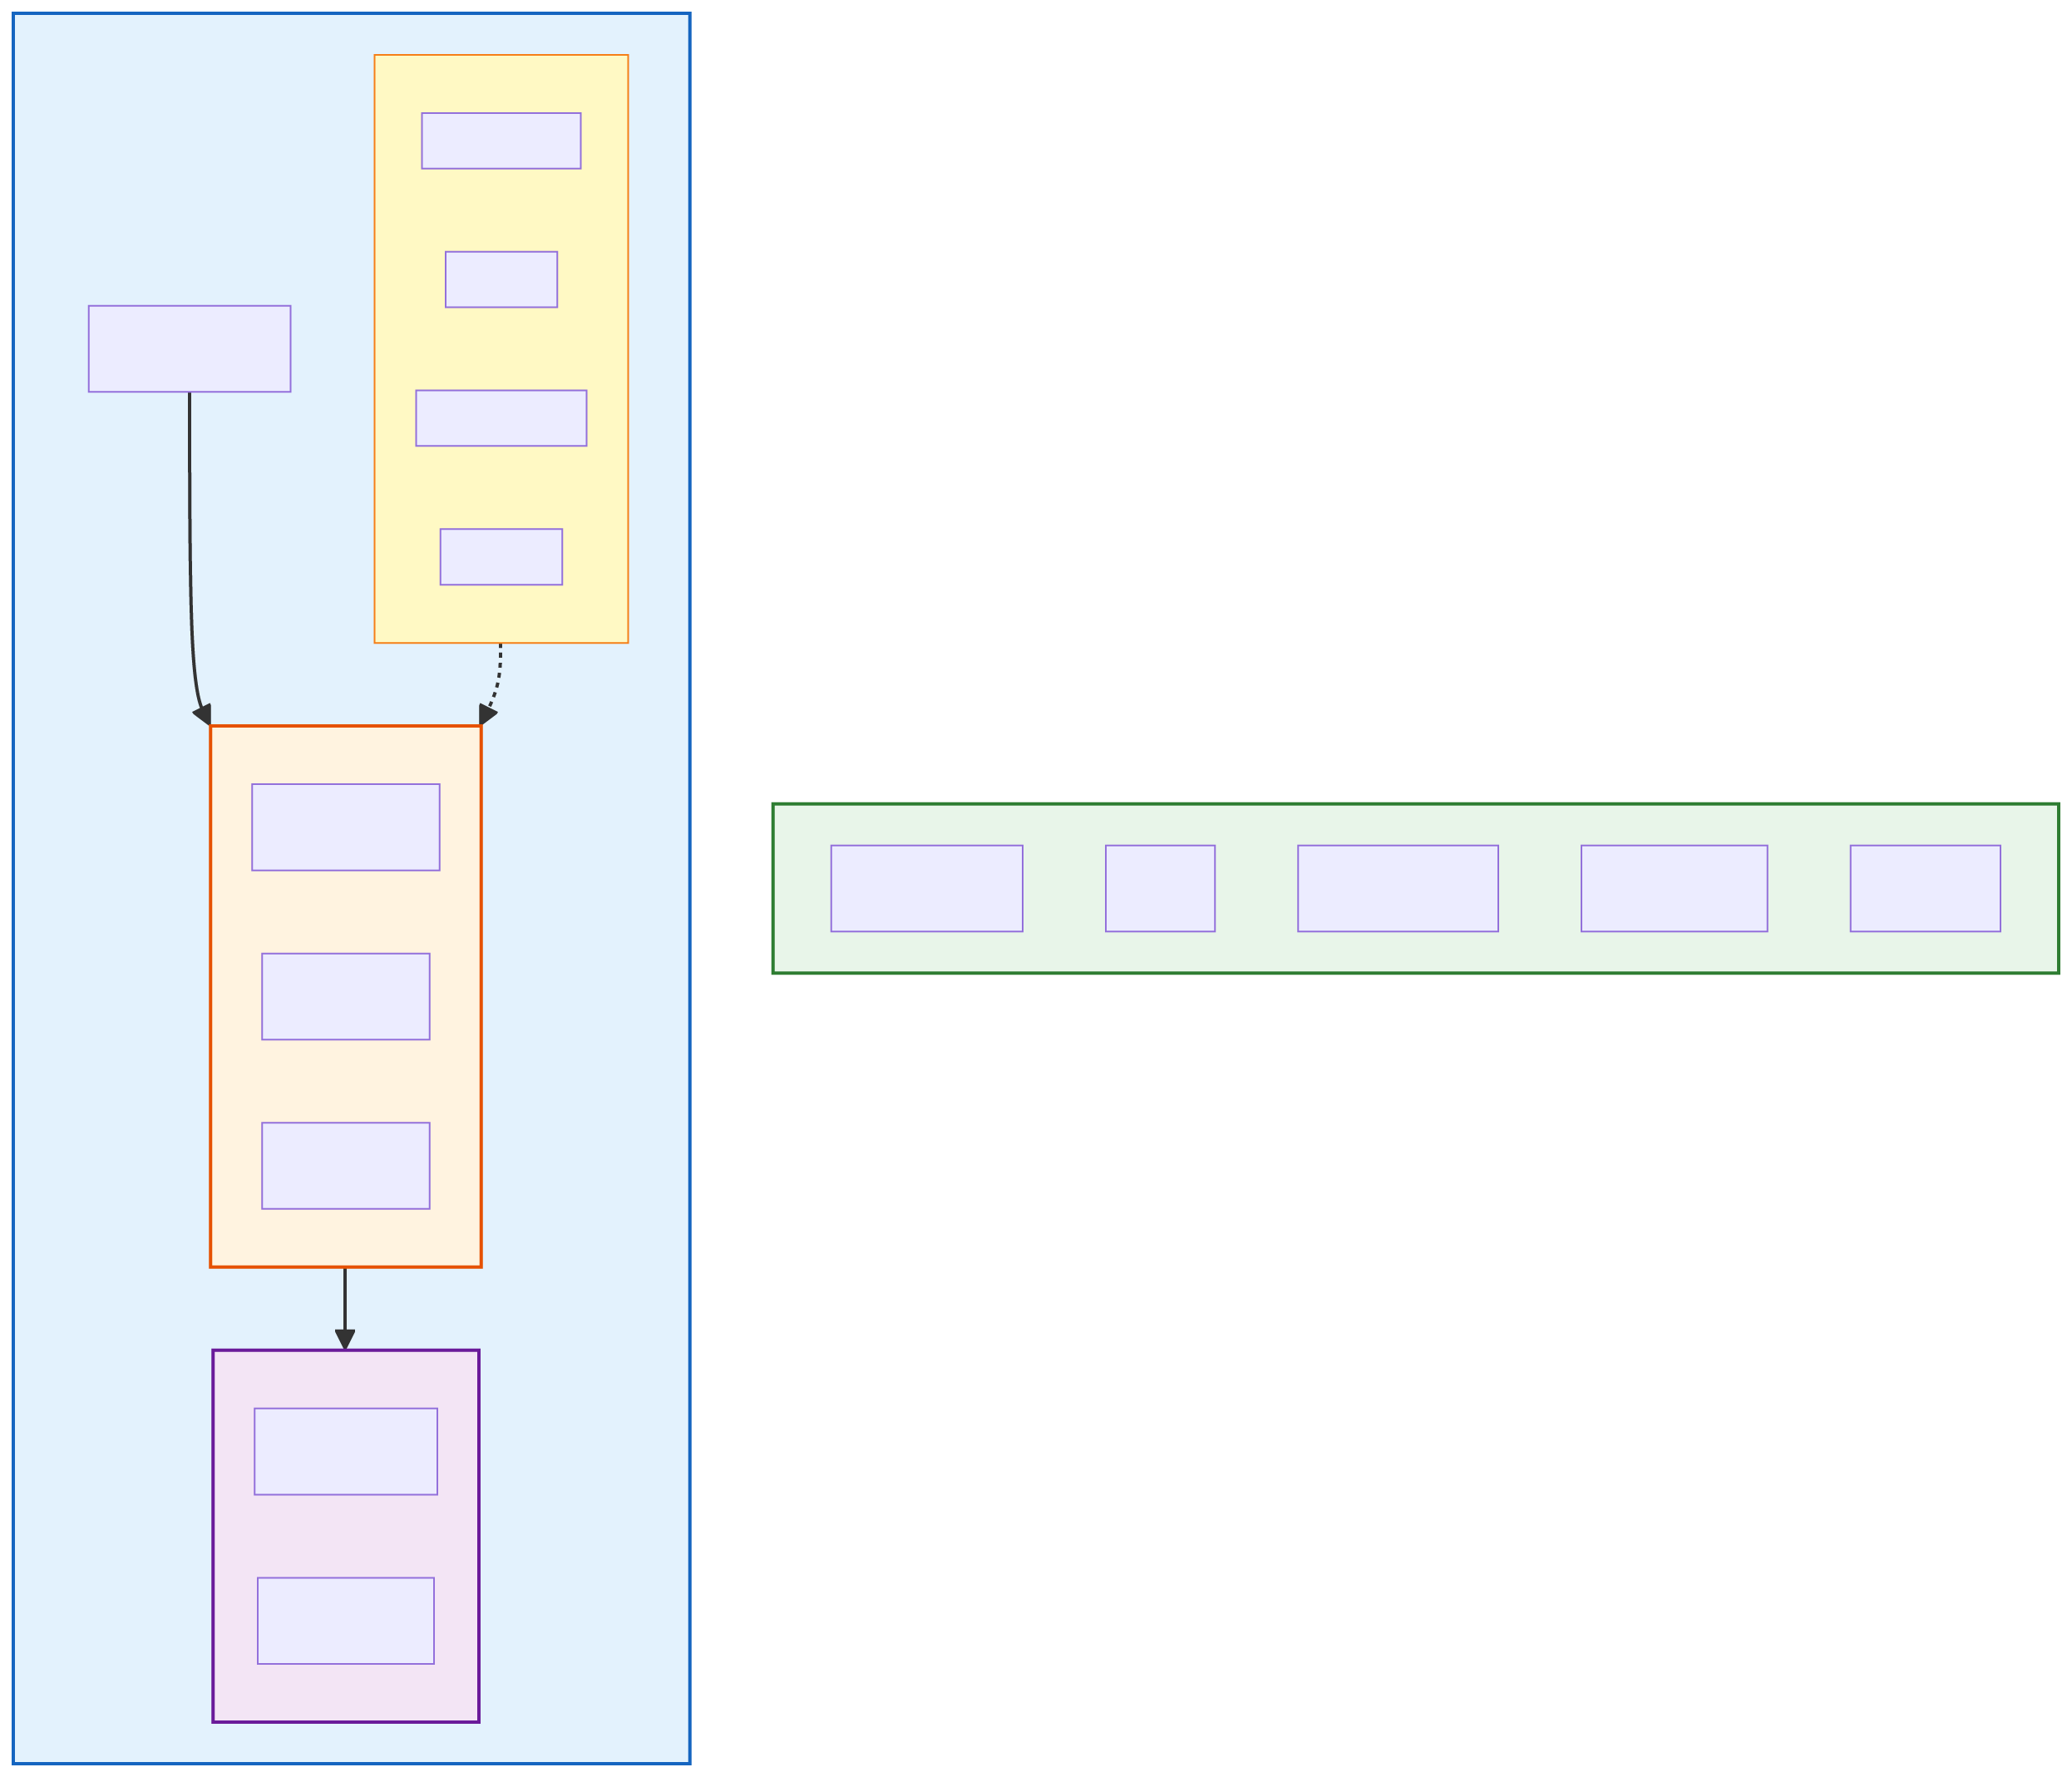
\includegraphics[width=\columnwidth]{figure_4_deployment_architecture.png}}
\caption{Deployment architecture showing Docker Compose for local development and K3s Kubernetes for production on GCP.}
\label{fig:deployment}
\end{figure}

\subsection{User Interface}
The platform provides interfaces for: IELTS Hub (4-stage learning journey), exam practice, AI grading results with detailed feedback, Vocab Lab flashcards, pronunciation checker, shadowing/dictation, and grammar lessons.



\subsection{SM-2 Spaced Repetition Evaluation}
A stochastic simulation was conducted over $N=50$ review iterations with three user profiles: User~A (90\% accuracy), User~B (60\%), and User~C (30\%).

\subsubsection{Interval Progression}
Fig.~\ref{fig:sm2_interval} presents the interval progression, Fig.~\ref{fig:sm2_ease} shows the ease factor evolution, and Fig.~\ref{fig:sm2_states} illustrates the state transition patterns.

\begin{figure}[htbp]
\centerline{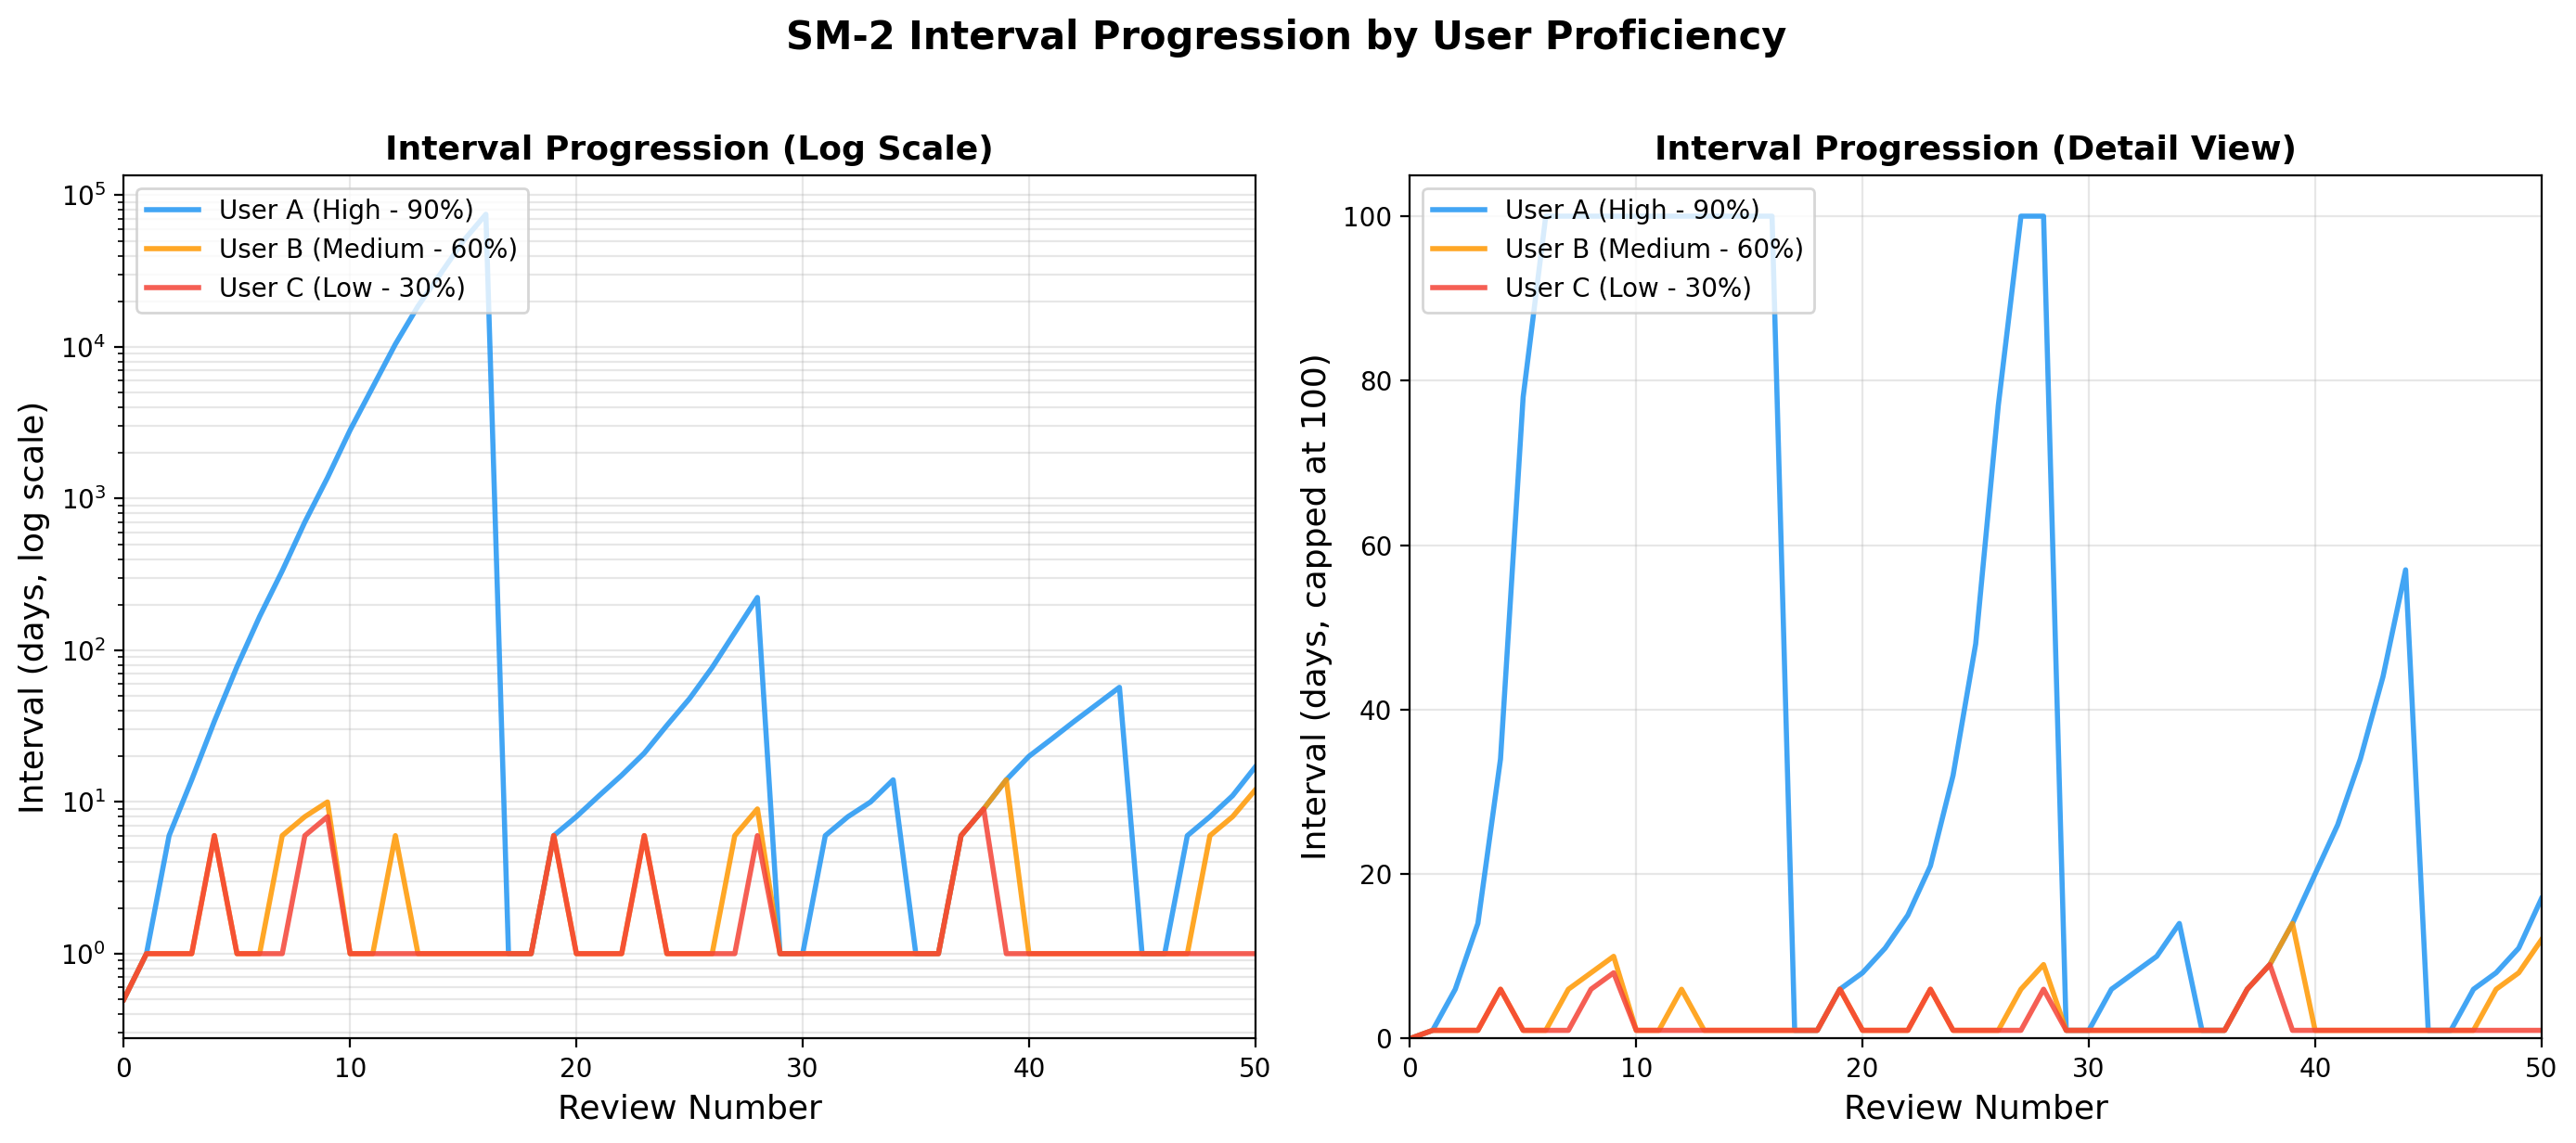
\includegraphics[width=\columnwidth]{sm2_interval_progression.png}}
\caption{SM-2 interval progression over 50 reviews for three user profiles: User~A (90\% accuracy), User~B (60\%), and User~C (30\%).}
\label{fig:sm2_interval}
\end{figure}

\begin{figure}[htbp]
\centerline{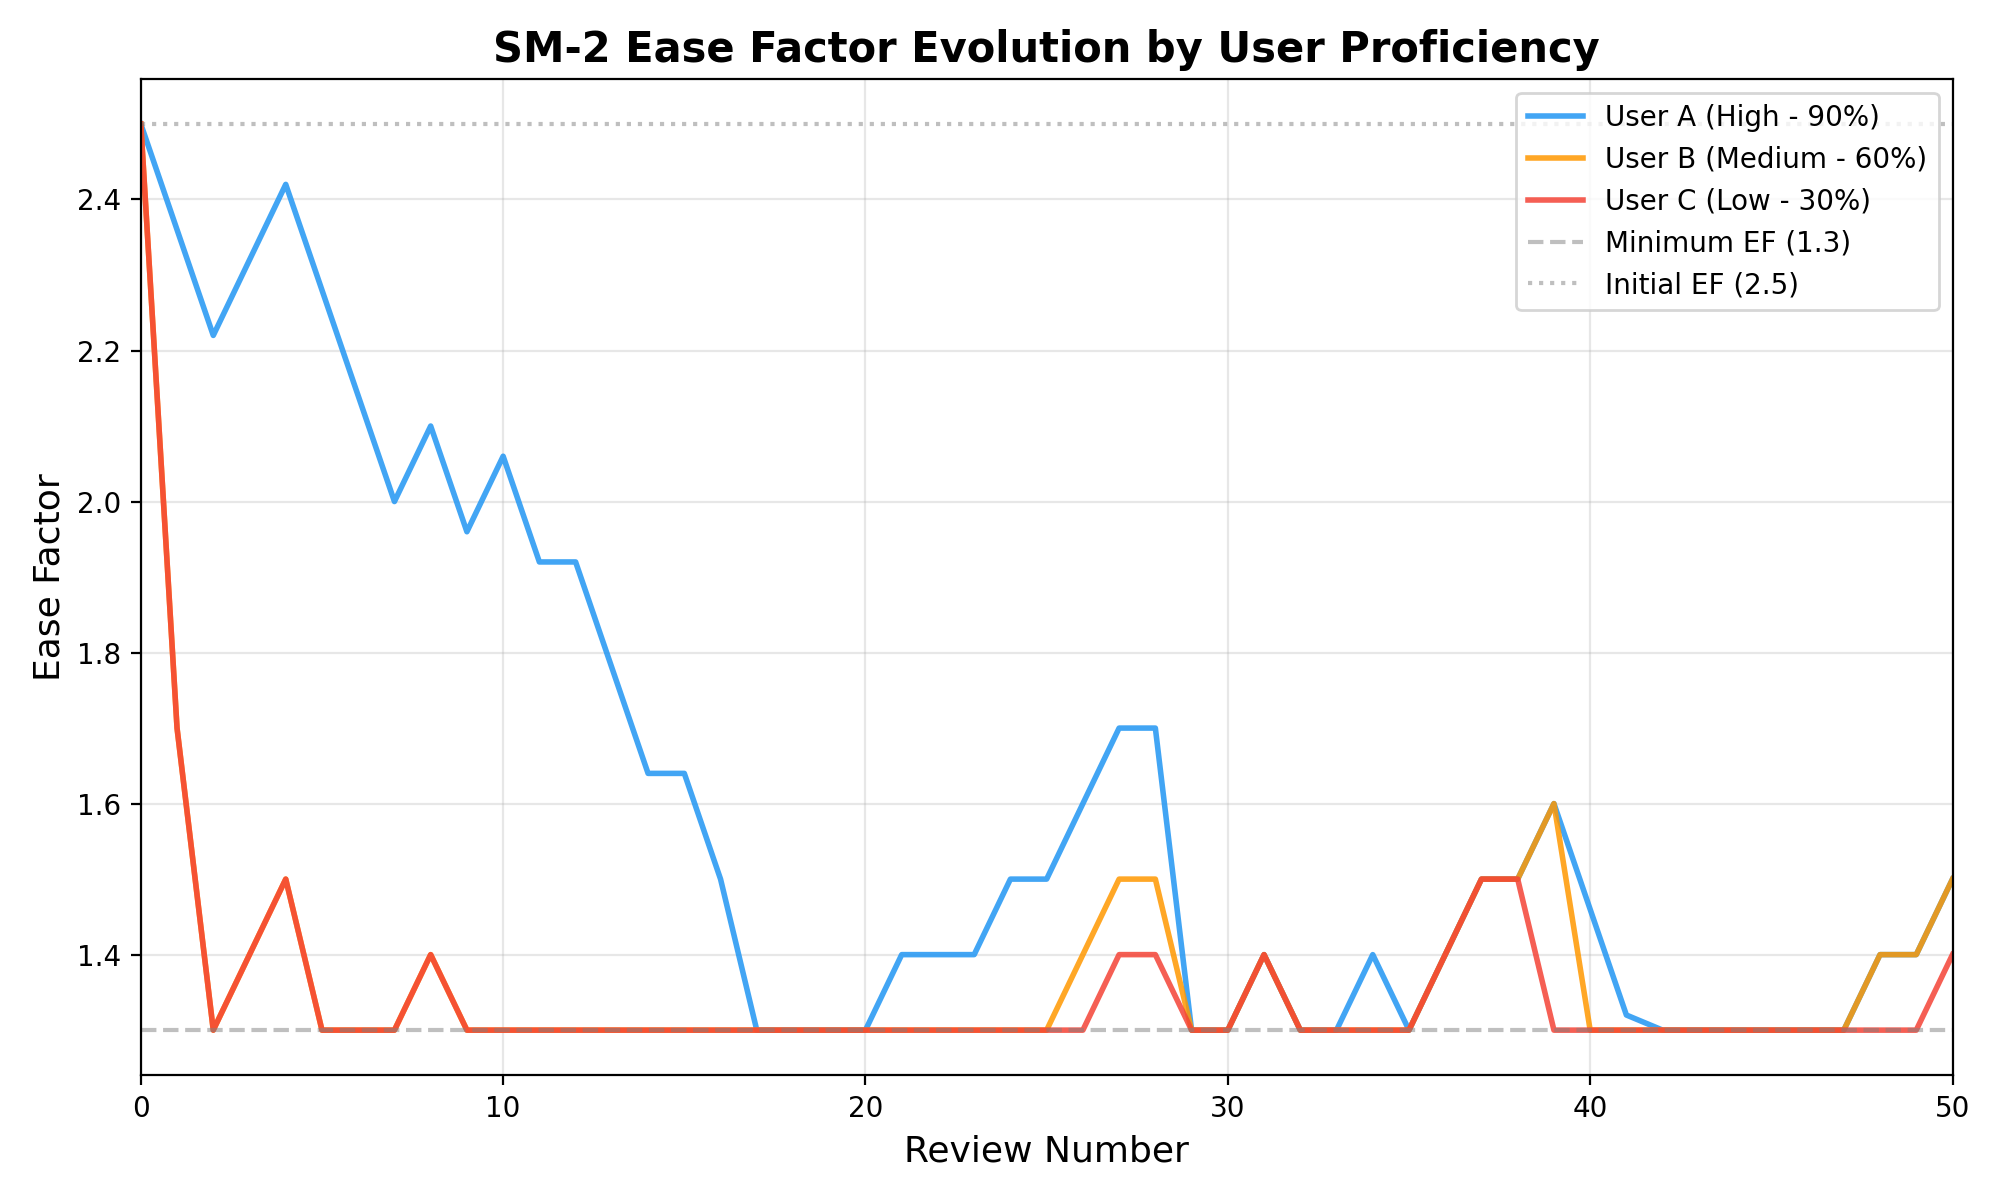
\includegraphics[width=\columnwidth]{sm2_ease_factor.png}}
\caption{SM-2 ease factor evolution showing how the algorithm adapts difficulty based on user performance.}
\label{fig:sm2_ease}
\end{figure}

\begin{figure}[htbp]
\centerline{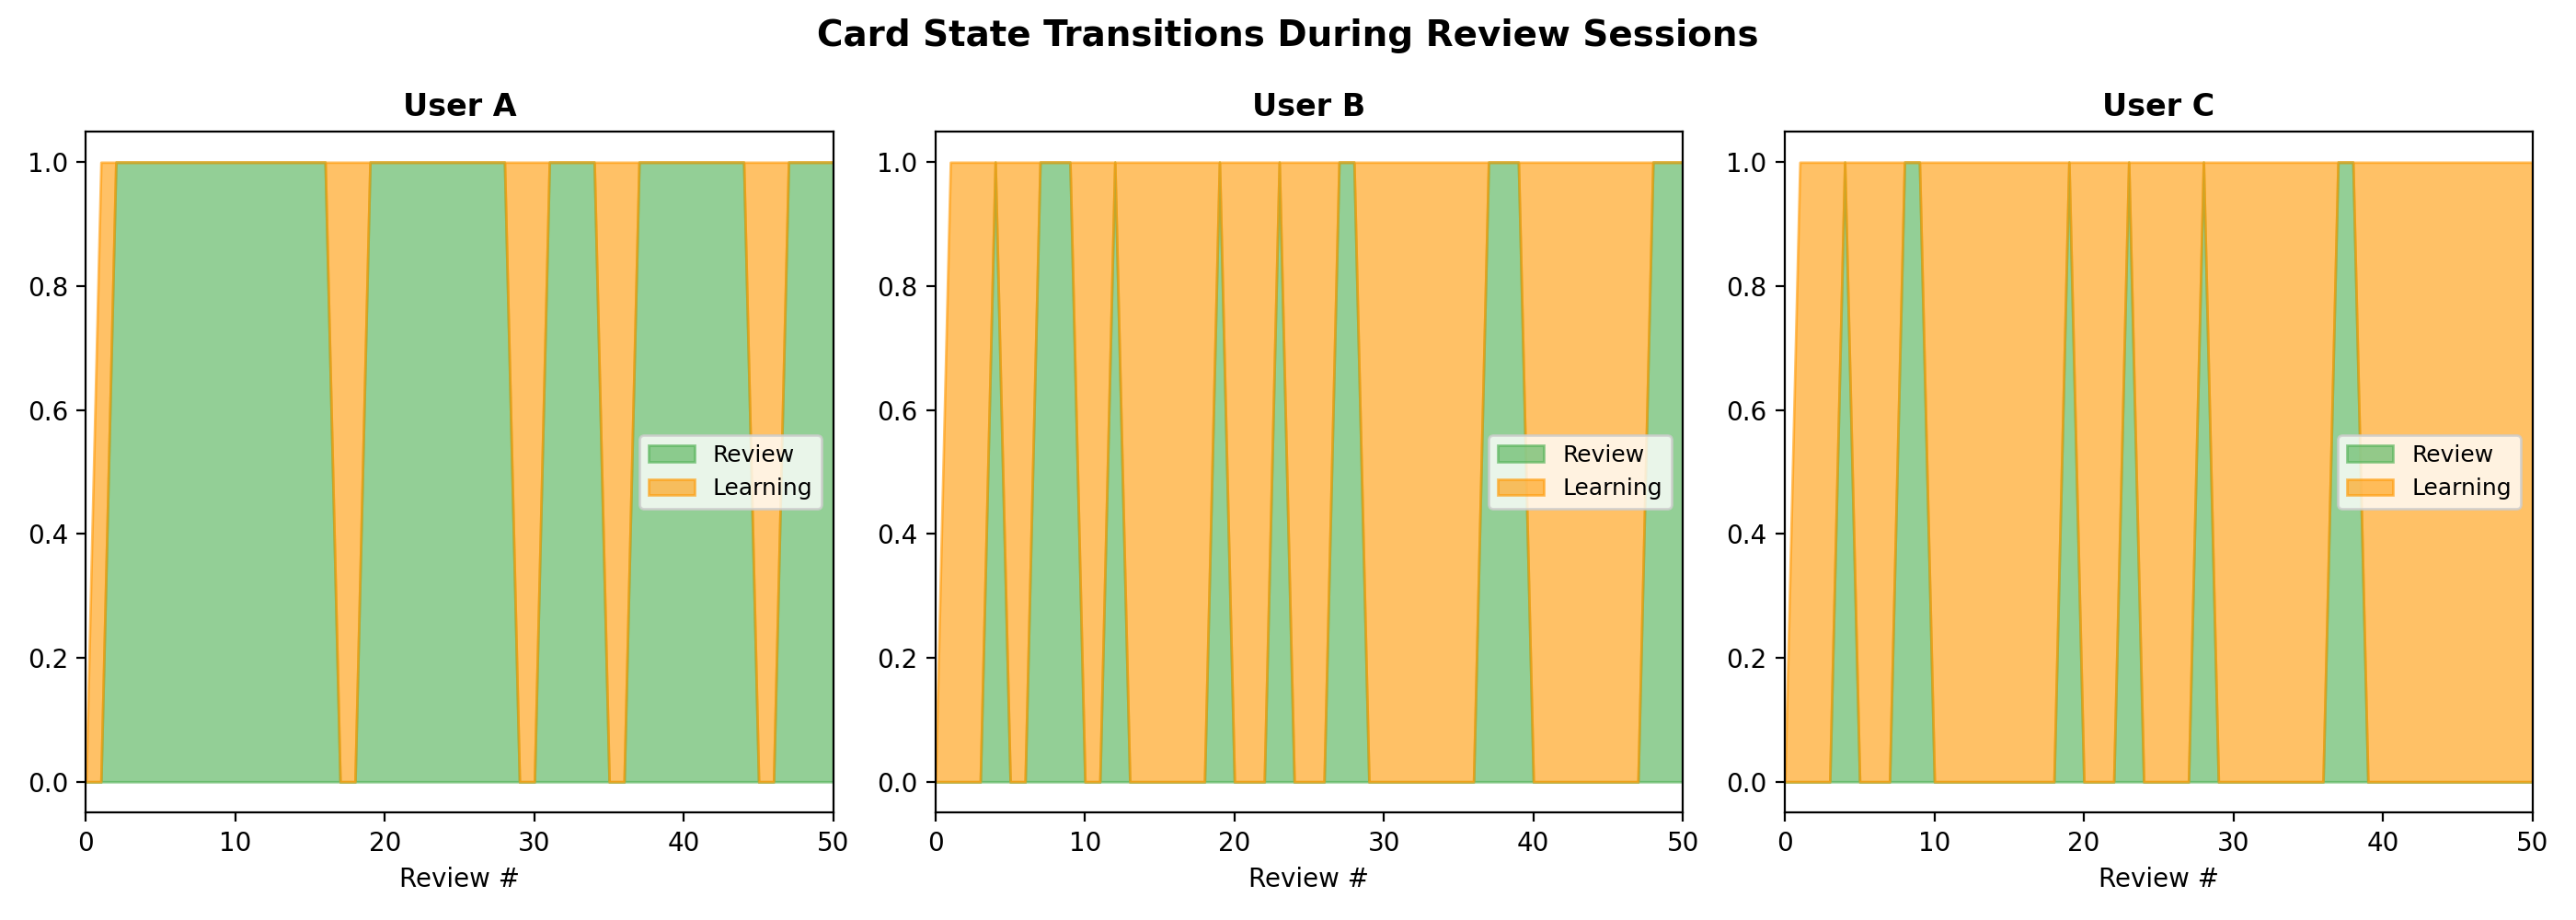
\includegraphics[width=\columnwidth]{sm2_state_transitions.png}}
\caption{SM-2 card state transitions (NEW $\rightarrow$ LEARNING $\rightarrow$ REVIEW) across user proficiency levels.}
\label{fig:sm2_states}
\end{figure}

User~A (46/50 correct) achieves exponential interval growth, reaching a maximum of 74,922 days and entering the REVIEW state 41/50 times. User~B (28/50 correct) reaches a maximum interval of 14 days with 15 REVIEW entries. User~C (20/50 correct) remains at a final interval of 1~day with only 8 REVIEW entries. All ease factors decline from the initial 2.5, with User~A stabilizing at 1.50 and User~C converging to 1.40 near the minimum bound. Table~\ref{fig:sm2_summary} provides a quantitative summary.

\begin{figure}[htbp]
\centerline{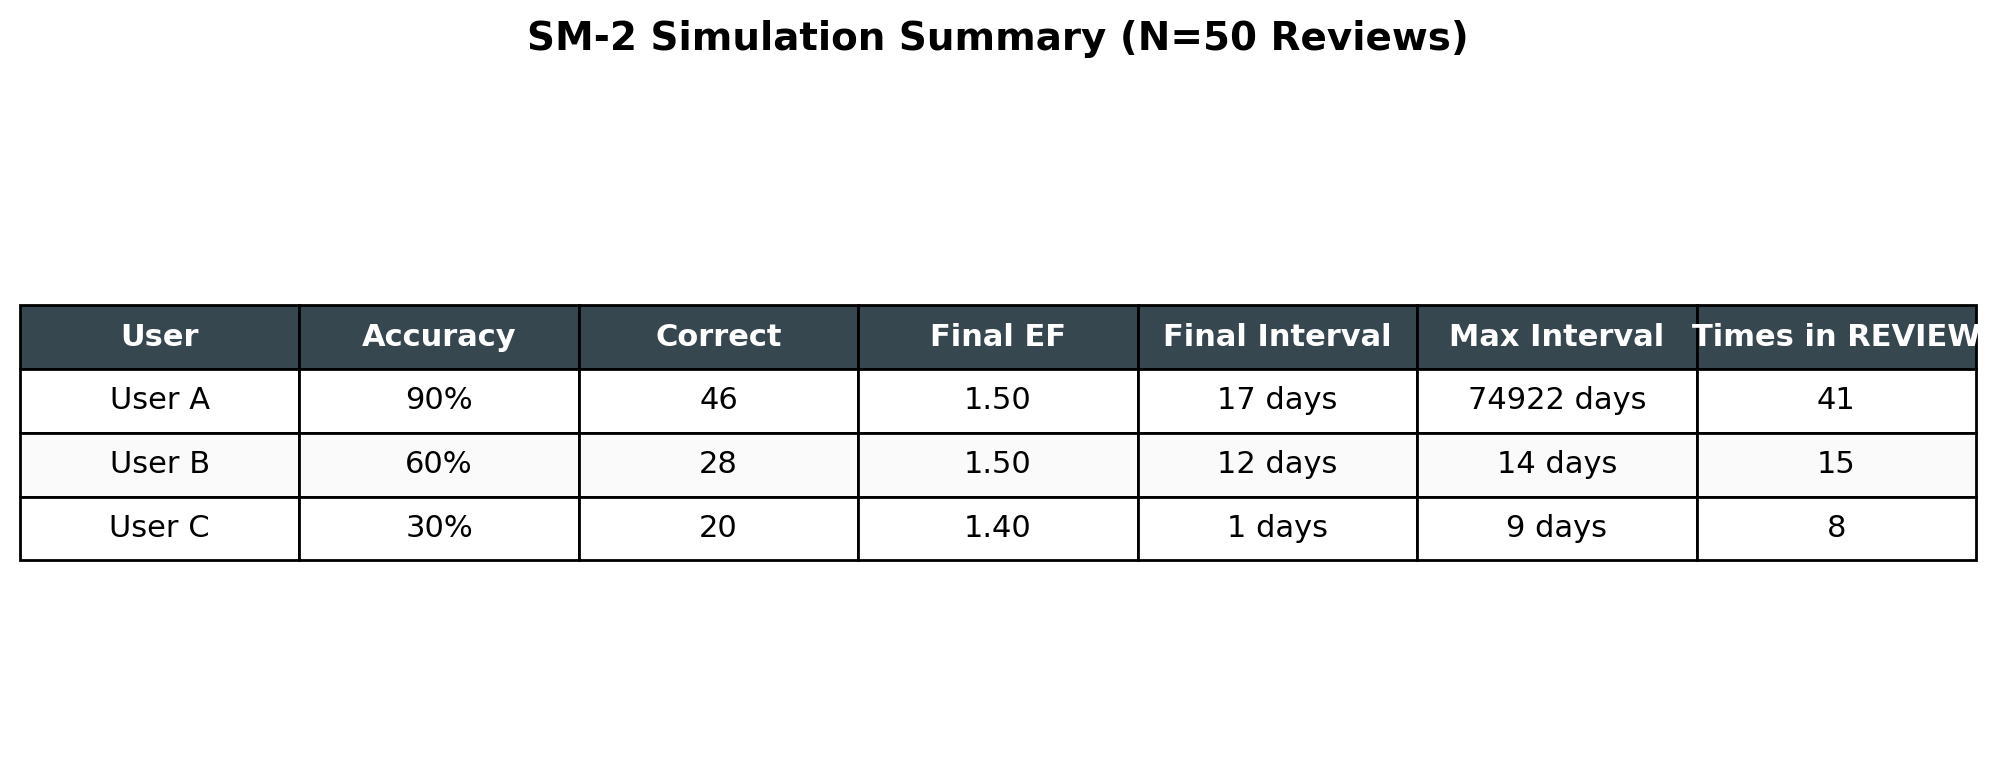
\includegraphics[width=\columnwidth]{sm2_summary_table.png}}
\caption{Summary statistics for the SM-2 simulation across the three user profiles.}
\label{fig:sm2_summary}
\end{figure}

\subsubsection{Discrimination Capability}
The SM-2 penalty mechanism ($q < 3$ triggers reset) effectively prevents progression through insufficient knowledge, ensuring items are reviewed at high frequency until mastery.

\subsection{Pronunciation Scoring Evaluation}
51 pronunciation attempt pairs were tested across three difficulty levels. The results are presented in Fig.~\ref{fig:pron_dist}--\ref{fig:pron_edit}.

\begin{figure}[htbp]
\centerline{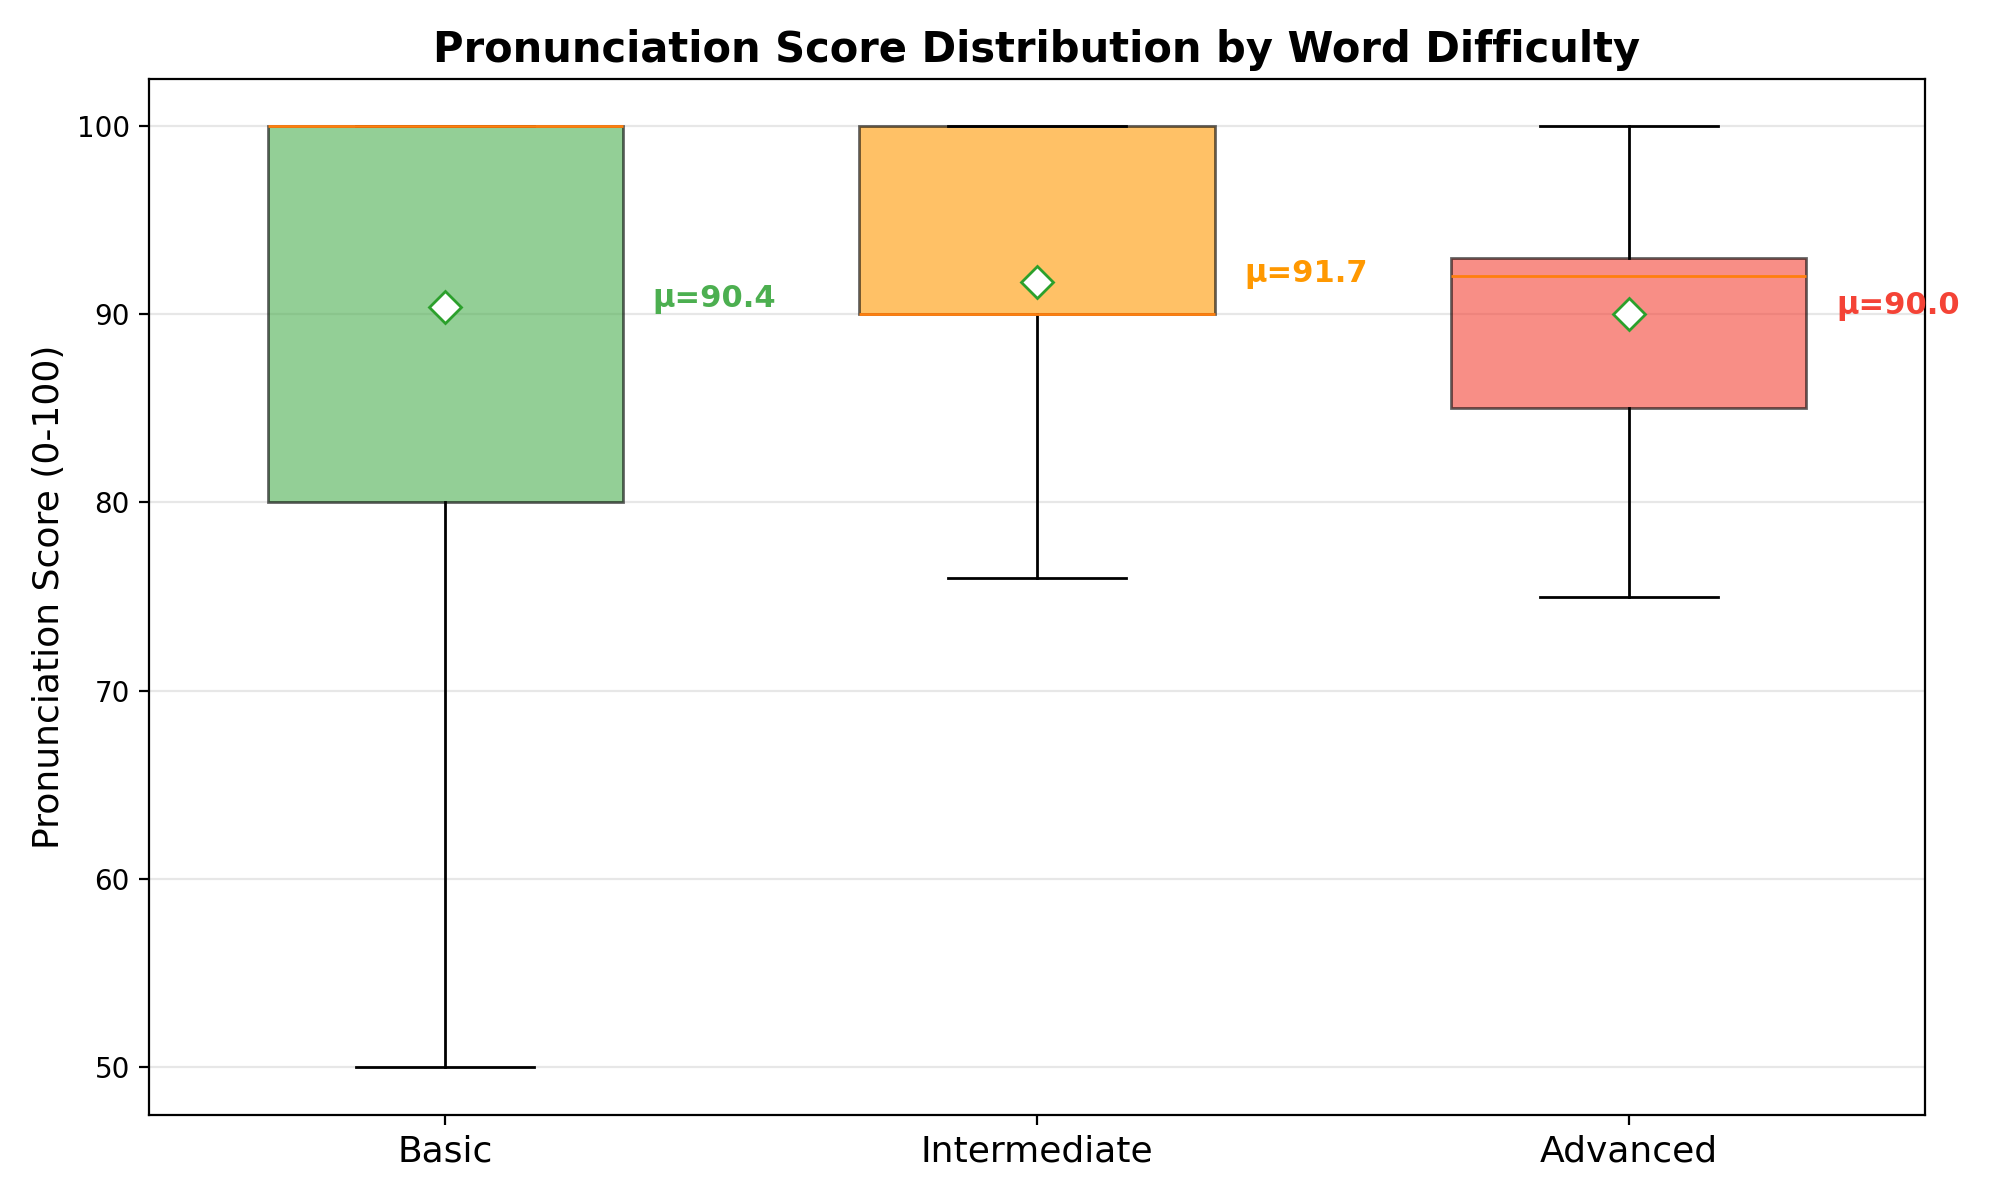
\includegraphics[width=\columnwidth]{pronunciation_score_distribution.png}}
\caption{Pronunciation score distribution by word difficulty level (Basic, Intermediate, Advanced).}
\label{fig:pron_dist}
\end{figure}

\begin{figure}[htbp]
\centerline{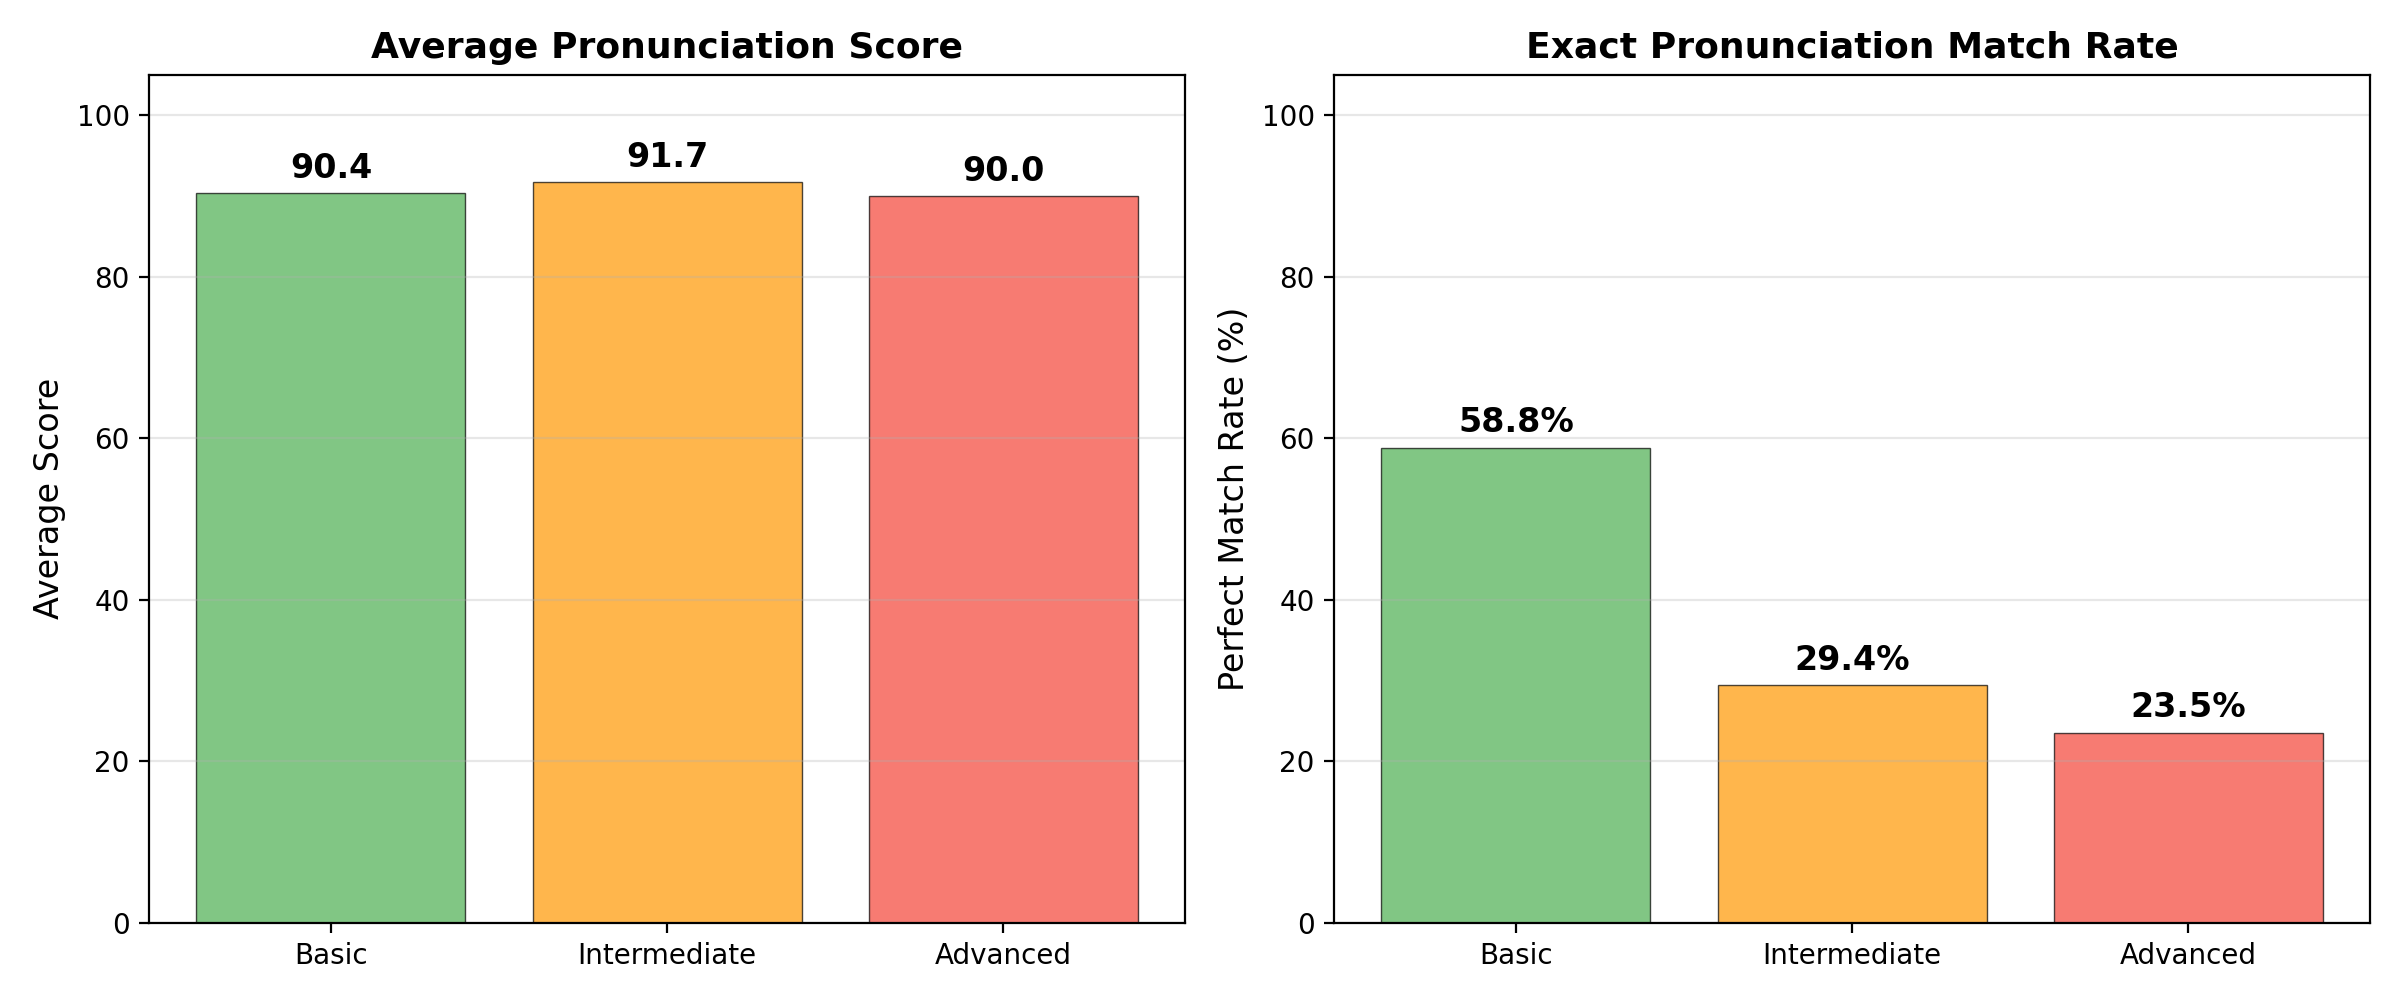
\includegraphics[width=\columnwidth]{pronunciation_accuracy_bars.png}}
\caption{Pronunciation accuracy comparison across difficulty levels showing mean scores and perfect match rates.}
\label{fig:pron_accuracy}
\end{figure}

\begin{figure}[htbp]
\centerline{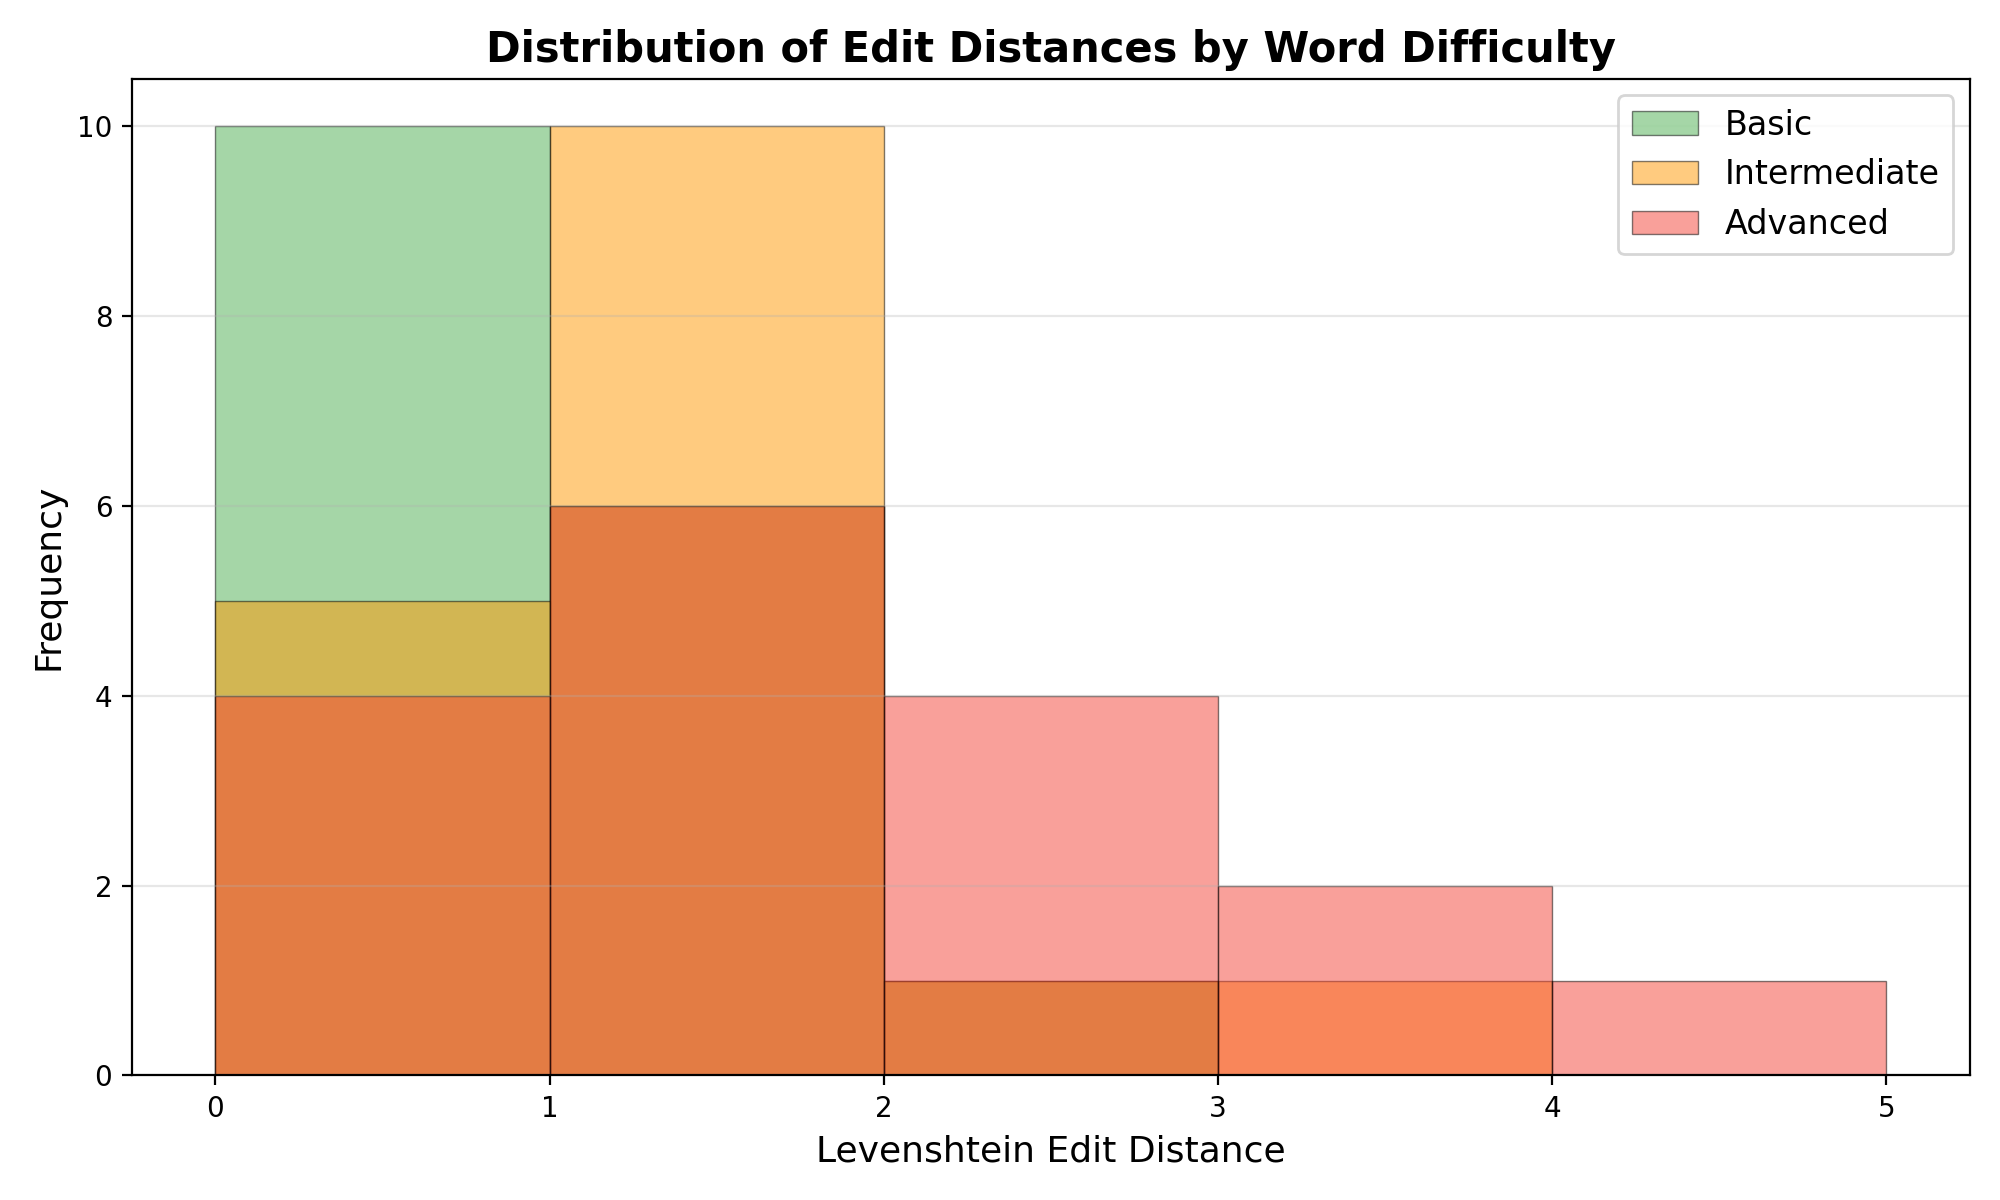
\includegraphics[width=\columnwidth]{pronunciation_edit_distance.png}}
\caption{Levenshtein edit distance distribution between transcribed and target words across difficulty categories.}
\label{fig:pron_edit}
\end{figure}

Basic words (17 samples): $\mu=90.4\%$, $\sigma=13.5$, 58.8\% perfect match rate. Intermediate (17 samples): $\mu=91.7\%$, $\sigma=6.7$, 29.4\% perfect match. Advanced (17 samples): $\mu=90.0\%$, $\sigma=7.5$, 23.5\% perfect match. The declining perfect match rate validates difficulty-level sensitivity.

\subsection{System Performance}
Table~\ref{tab:performance} summarizes response times.

\begin{table}[htbp]
\caption{System Performance Characteristics}
\label{tab:performance}
\centering
\begin{tabular}{lcc}
\toprule
\textbf{Operation} & \textbf{Avg. Time} & \textbf{Method} \\
\midrule
Listening/Reading grading & $<$100 ms & Sync \\
Writing AI grading & 8--15 s & Sync (LLM) \\
Speaking AI grading & 10--25 s & Sync (Whisper+LLM) \\
Pronunciation check & 3--8 s & Async (RabbitMQ) \\
Non-AI API response & 20--80 ms & Cached (Redis) \\
\bottomrule
\end{tabular}
\end{table}

% ============================================================
\section{Conclusion and Future Work}
% ============================================================

This paper presented IELTS Master English AI, a comprehensive IELTS preparation platform built on an Event-Driven Hybrid Architecture. The key contributions include: (1) clean separation of business logic from AI processing via RabbitMQ, (2) local Faster-Whisper speech processing as a cost-effective alternative to cloud APIs, (3) LLM-based Writing and Speaking grading with structured rubric output, and (4) a comprehensive learning pipeline with SM-2 spaced repetition vocabulary.

Future work includes: teacher analytics dashboards, on-device ML for offline mobile use, multi-test support (TOEFL, PTE), advanced learning analytics, and social/gamification features.

% ============================================================
% REFERENCES
% ============================================================

\begin{thebibliography}{15}

\bibitem{ielts_stats}
IELTS Partners, ``IELTS: Test Statistics,'' 2024. [Online]. Available: \url{https://www.ielts.org/research/test-statistics}

\bibitem{faster_whisper}
SYSTRAN, ``Faster-Whisper: Faster Whisper transcription with CTranslate2,'' GitHub, 2023. [Online]. Available: \url{https://github.com/SYSTRAN/faster-whisper}

\bibitem{richards_arch}
M. Richards, \textit{Software Architecture Patterns}. O'Reilly Media, 2015.

\bibitem{nestjs_docs}
K. Mysliwiec, ``NestJS Documentation,'' 2024. [Online]. Available: \url{https://docs.nestjs.com}

\bibitem{fastapi_docs}
S. Ramirez, ``FastAPI Documentation,'' 2024. [Online]. Available: \url{https://fastapi.tiangolo.com}

\bibitem{gpt3}
T. Brown \textit{et al.}, ``Language Models are Few-Shot Learners,'' in \textit{NeurIPS}, 2020.

\bibitem{sm2}
P. A. Wozniak, ``Application of a computer to improve the results obtained in working with the SuperMemo method,'' 1990.

\bibitem{levenshtein}
V. I. Levenshtein, ``Binary codes capable of correcting deletions, insertions, and reversals,'' \textit{Soviet Physics Doklady}, vol. 10, no. 8, pp. 707--710, 1966.

\bibitem{whisper_paper}
A. Radford \textit{et al.}, ``Robust Speech Recognition via Large-Scale Weak Supervision,'' in \textit{ICML}, 2023.

\bibitem{nextjs}
M. Riva, \textit{Real-World Next.js}. Packt Publishing, 2022.

\bibitem{react_native}
O'Reilly Media, ``Learning React Native,'' 2020.

\bibitem{rabbitmq}
RabbitMQ, ``RabbitMQ Documentation,'' 2024. [Online]. Available: \url{https://www.rabbitmq.com/documentation.html}

\bibitem{redis}
Redis, ``Redis Documentation,'' 2024. [Online]. Available: \url{https://redis.io/documentation}

\bibitem{prisma}
Prisma, ``Prisma ORM Documentation,'' 2024. [Online]. Available: \url{https://www.prisma.io/docs}

\bibitem{reference_paper}
[Authors], ``Social Network Platform Supporting English Learning and Multimedia Communication,'' in \textit{Student Scientific Research Communication}, vol. I, 2025.

\end{thebibliography}

\end{document}
